% !TeX spellcheck = en_US
\documentclass{article} % For LaTeX2e
\usepackage{nips15submit_e,times}
\usepackage{hyperref}
\usepackage{url}
\usepackage{amsmath}
\usepackage{graphicx} 
\usepackage{multirow}
\usepackage{subcaption}
%\documentstyle[nips14submit_09,times,art10]{article} % For LaTeX 2.09


\title{Comparing two Convolution Neural Networks for Image Classification}

	
\author{
	Shikhar Vashishth  \\
	M.Tech CSA\\
	IISc Bangalore \\
	\texttt{shikhar.vashishth@csa} \\
}



% The \author macro works with any number of authors. There are two commands
% used to separate the names and addresses of multiple authors: \And and \AND.
%
% Using \And between authors leaves it to \LaTeX{} to determine where to break
% the lines. Using \AND forces a linebreak at that point. So, if \LaTeX{}
% puts 3 of 4 authors names on the first line, and the last on the second
% line, try using \AND instead of \And before the third author name.

\newcommand{\fix}{\marginpar{FIX}}
\newcommand{\new}{\marginpar{NEW}}

\nipsfinalcopy % Uncomment for camera-ready version

\begin{document}

	\maketitle
	
	\begin{abstract}
		The project compares two popular Convolution Neural Network (CNN) architectures: AlexNet and ZFNet which have won ImageNet LSVRC challenge in the year 2012 and 2013 by a considerable margin. Both the architectures have been a breakthrough in the field of deep learning. The goal of this project is to explore these successful architectures and look into the working of their each individual layer using a technique called Deconvolution and explore the evolution of ZFNet from AlexNet. It also proposes a new way of visualizing ConvNets using a novel technique called DeNet.
	\end{abstract}
	
	\section{Introduction}
	The concept of Neural Networks has been around for several decades but in the year 2012 the real potential of this model was actually admitted and acknowledged by the entire world. The Convolutional Neural Network architecture, \textbf{AlexNet}, proposed by Alex Krizhevsky et al [1] was the first breakthrough architecture which won the ImageNet LSVRC [3] 2012 challenge with a huge margin. It won the challenge with an error rate of \textbf{15.3 \%} while the second-best contest entry achieved an error rate of \textbf{26.2 \%} on classification task of 1.2 million images into 1000 different categories. Thus, the model was the state-of-the-art at that time. AlexNet although was the best among all the known models but still the reason for its performance was unknown. In the year 2013, [3] Mattew D. Zeiler et al came up with a way to understand the working of CNN architectures by giving a method for visualizing the activations of convolution layers in the network. The method was called \textbf{Deconvolution} [5] because it allows to project the output of convolution layers back to the pixel domain. Based on their analysis of AlexNet using their new technique, they discovered certain loopholes in AlexNet architecture which were rectified and thus gave rise to a new CNN architecture, ZFNet, which won the ImageNet LSVRC challenge in 2013. This project explores both of these architectures in detail and discusses the technique, deconvolution which can be used for visualizing any convolution neural network. The project also proposes a novel method for visualizing CNN networks called \textbf{DeNet}, which involves transforming the final vector denoting the category of an image back to the pixel domain by reversing the operations of every layer in the network systematically. 
	
	\section{Convolution Neural Networks}
	Convolution Neural Networks are an extension of standard Neural Networks, which are specifically designed to process multi-dimensional data. Just like Neural Networks, CNNs also are based on transforming inputs through a series of hidden layers, but compared to NNs they are much more efficient and have considerably fewer parameters to train. Performance of CNNs is much better than NNs on images because they make use of the spatial structure of the image which is left unexploited by NNs. CNN architecture is mainly composed of three layers, namely convolution, pooling and fully-connected layers, which are intelligently stacked together to give the desired results.
	
	\subsection{Convolution Layer}
	Convolution layers are composed of several filters which are convolved with the image to produce the output. On training, these filters become specialized to look for some specific features in the image data. These filters are the main source of drastic reduction in CNN parameters because the same set of filters is shared across the entire layer. Each convolution layer has several hyperparameters which include number of filters $K$, filter size $F$ (dimensions of a filter), stride $S$ with which filters are convolved with the image and padding size $P$, which is appended to the image before convolving. These parameters decide the output dimensions of the convolution layer according to the following formulas.
		$$  W_2 = (W_1 - F + 2P)/S + 1 $$
		$$  H_2 = (H_1 - F + 2P)/S + 1 $$
		$$  D_2 = K $$
		
	Here, $ W_1 \times H_1 \times D_1$  is the input dimensions and $ W_2 \times H_2 \times D_2$  is the output dimensions. 
	
	\begin{figure}[h]
		\centering
		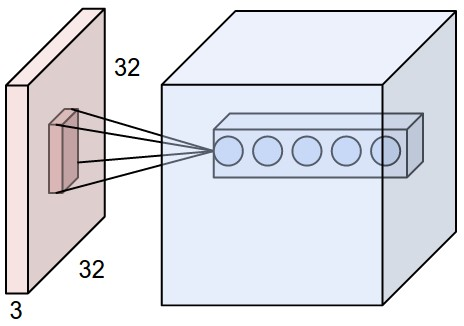
\includegraphics[width=5cm]{Images/conv_layer.jpeg}
		\caption{Convolution Layer}
	\end{figure}

	Every convolution layer is followed by an activation function which adds non-linearity in CNN. Few of the activation functions are listed below:
	\begin{center}
		\begin{tabular}{ c c c c c c }
			& & & & &\\
			Sigmoid &:& $f(\eta)$ &$=$& $a / (1+e^{-b\eta})$ & $a,b>0$\\
			& & & & &\\
			Tan hyperbolic &:& $f(\eta)$ &$=$& $atanh(b\eta)$ & $a,b>0$\\
			& & & & &\\
			ReLU &:& $f(\eta)$ &$=$& $max(o,\eta)$ &\\
			& & & & &\\
			Leaky ReLU &:& $f(\eta)$ &$=$& $max(\alpha \eta, \eta)$ & $\alpha >0$\\
			& & & & &\\
		\end{tabular}
	\end{center}

	
	\subsection{Pooling layers}
	Pooling layers are generally stacked after a convolution layer for summarizing its output by downsampling. Downsampling allows network to keep only the local information of features while forgetting the locality information. Max-pooling is the most commonly used pooling layer. Other than that, average pooling and L2-norm pooling are also used in some architectures. Pooling layers make convnets invariant to translation of input which is very useful in image recognition problems. Hyperparameters of layer include stride $S$ and its spatial extent $F$. They decide the dimensions of output according to the following formulas: 
	
		$$  W_2 = (W_1 - F )/S + 1 $$
		$$  H_2 = (H_1 - F )/S + 1 $$
		%\begin{figure}[h]
	%		\centering
%			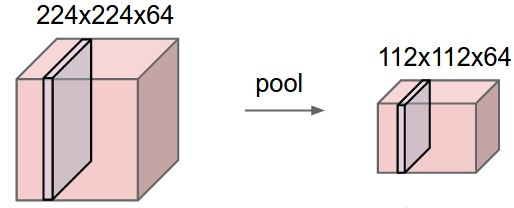
\includegraphics[width=5cm]{pool_layer.jpeg}
%			\caption{Pooling Layer}
%		\end{figure}
	
	\subsection{Fully-Connected Layers}
	Every convolution neural network ends with a series of fully-connected layers which are the regular layers from the standard Neural Networks. The number of neurons in the final output layer is equal to the number of classes in the given classification problem.
	
	
	\section{AlexNet}
	AlexNet [1] is the first most successful Convolution Neural Network architecture for Image classification, which was introduced by Alex Krizhevsky, I. Sutskerver and G. Hinton in the year 2012. The network is composed of five convolution layers and three fully connected layers, making it a CNN with 60 million trainable parameters. In each layer, instead of the standard sigmoid activation function, a new activation function called ReLU was used which made the network less vulnerable to the vanishing gradient problem and faster to train. The network also consists of normalization layers after few (first two) convolution layers which further improved its performance by making model invariant to brightness. 
	
	The original architecture of the model is shown in the Figure \ref{alexnet_old}. Because of the non-availability of highly efficient GPUs at that time, the original model was split into two different streams for reducing the training time. In this project, I have used the single stream architecture of the AlexNet which is shown in the Figure \ref{alexnet_new}.
	
	\begin{figure}[h]
		\centering
		\fbox{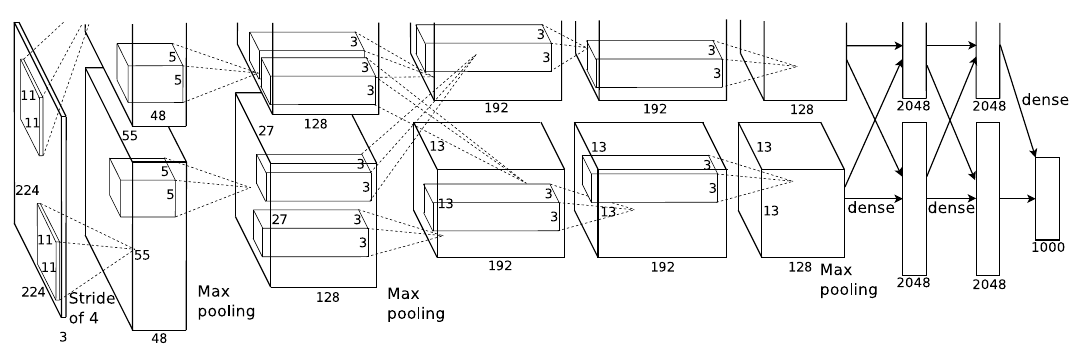
\includegraphics[width=12cm]{Images/alexnet_old2}}
		\caption{AlexNet Original architecture}
		\label{alexnet_old}
	\end{figure}

	\begin{figure}[h]
		\centering
		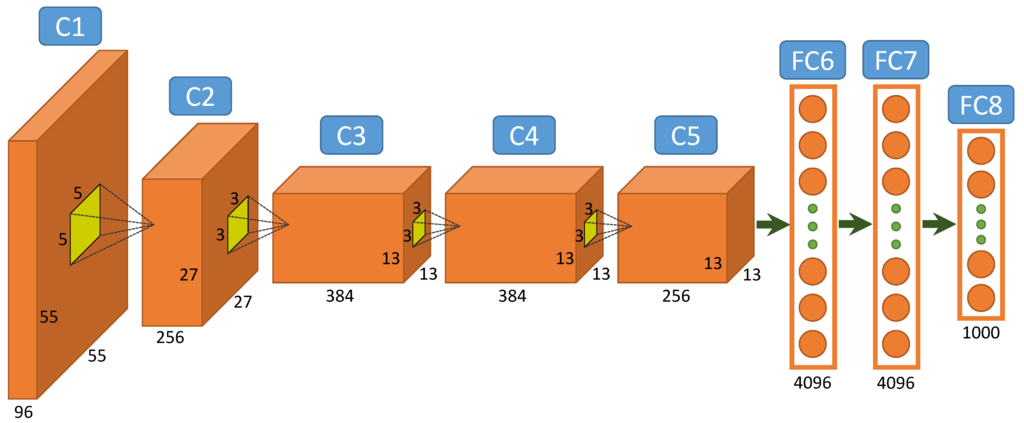
\includegraphics[width=12cm]{Images/alexnet_new2}
		\caption{AlexNet architecture}
		\label{alexnet_new}
	\end{figure}

	\subsection*{Details of AlexNet architecture:}
	\begin{enumerate}
		\item \textbf{Input:} $[227 \times 227 \times 3]$ dimensional
		\item \textbf{Conv1:} 96 filters of $[11 \times 11]$ size with stride 4 and padding 0
		\item \textbf{Max Pool 1:} $[3 \times 3]$ filter with stride $2$
		\item \textbf{Norm 1:} Normalization Layer
		\item \textbf{Conv2:} 256 filters of $[5 \times 5]$ size with stride 1 and padding 2
		\item \textbf{Max Pool 2:} $[3 \times 3]$ filter with stride $2$
		\item \textbf{Norm 2:} Normalization Layer
		\item \textbf{Conv3:} 384 filters of $[3 \times 3]$ size with stride 1 and padding 1
		\item \textbf{Conv4:} 384 filters of $[3 \times 3]$ size with stride 1 and padding 1
		\item \textbf{Conv5:} 256 filters of $[3 \times 3]$ size with stride 1 and padding 1
		\item \textbf{Max Pool 3:} $[3 \times 3]$ filter with stride $2$
		\item \textbf{Dense 1:} 4096 neurons (Dropout 0.5)
		\item \textbf{Dense 2:} 4096 neurons (Dropout 0.5)
		\item \textbf{Dense 3:} 1000 neurons
	\end{enumerate}


	\section{ZFNet}
	ZFNet [2] is an another Convolution Neural Network architecture, introduced by Zeiler and Ferger, which won the ImageNet LSVRC challenge in 2013. The architecture of ZFNet is very similar to that of AlexNet. Zeiler and Ferger just suggested few changes in the hyperparameters of AlexNet based on their analysis which increased its performance considerably. Through their work they tried to understand the reasons behind the magnificent performance of convnets. The architecture of ZFNet is shown in the Figure \ref{zfnet}.
	
	\begin{figure}[h]
		\centering
		\fbox{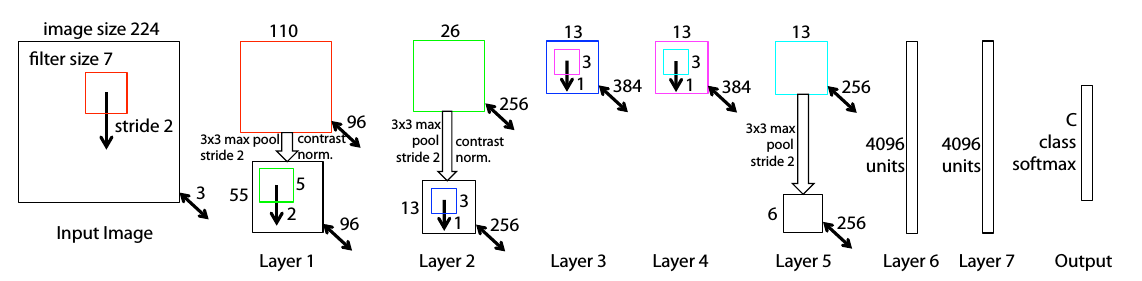
\includegraphics[width=\textwidth]{Images/zfnet}}
		\caption{ZFNet architecture}
		\label{zfnet}
	\end{figure}

	\subsection*{Details of ZFNet architecture:}
	\begin{enumerate}
		\item \textbf{Input:} $[224 \times 224 \times 3]$ dimensional
		\item \textbf{Conv1:} 96 filters of $[7 \times 7]$ size with stride 2 and padding 0
		\item \textbf{Max Pool 1:} $[3 \times 3]$ filter with stride $2$
		\item \textbf{Norm 1:} Normalization Layer
		\item \textbf{Conv2:} 256 filters of $[5 \times 5]$ size with stride 2 and padding 1
		\item \textbf{Max Pool 2:} $[3 \times 3]$ filter with stride $2$
		\item \textbf{Norm 2:} Normalization Layer
		\item \textbf{Conv3:} 384 filters of $[3 \times 3]$ size with stride 1 and padding 1
		\item \textbf{Conv4:} 384 filters of $[3 \times 3]$ size with stride 1 and padding 1
		\item \textbf{Conv5:} 256 filters of $[3 \times 3]$ size with stride 1 and padding 1
		\item \textbf{Max Pool 3:} $[3 \times 3]$ filter with stride $2$
		\item \textbf{Dense 1:} 4096 neurons (Dropout 0.5)
		\item \textbf{Dense 2:} 4096 neurons (Dropout 0.5)
		\item \textbf{Dense 3:} 1000 neurons
	\end{enumerate}

	\section{Deconvolution}
	We can see from the above description that ZFNet is actually AlexNet with slight change in hyperparameters. The main contribution of [2] was the use of the technique called \textbf{Deconvolution} [5]	 for visualizing convnets internal functioning. This technique helps to scientifically decide hyperparameters of convets rather than just depending on trial and errors. It allows to map activation of any convolution layer for an input image back to the pixel domain, highlighting the features which were actually captured by the layer for that input. For a fully trained network, the deconvolution is performed by designing layers which do the reverse of what the network does in the forward pass. For every convolution layer, a deconvolution layer is created and for every pooling layer an unpooling layer is created. To visualize the activation of a convolution layer $c$, for a given input $i$, firstly, a forward pass is performed and the activation corresponding to the layer $c$ is stored, rest are thrown away. Then, starting from $c$, by following the constructed deconvolution and unpooling layers the activation is mapped to the pixel domain. This process doesn't restore the original image because a lot of information is lost in unpooling and deconvolution operations, so only the features which were extracted by the layer $c$ are visible in the obtained image. The following figure summarizes the entire process.
	
	\begin{figure}[h]
		\centering
		\fbox{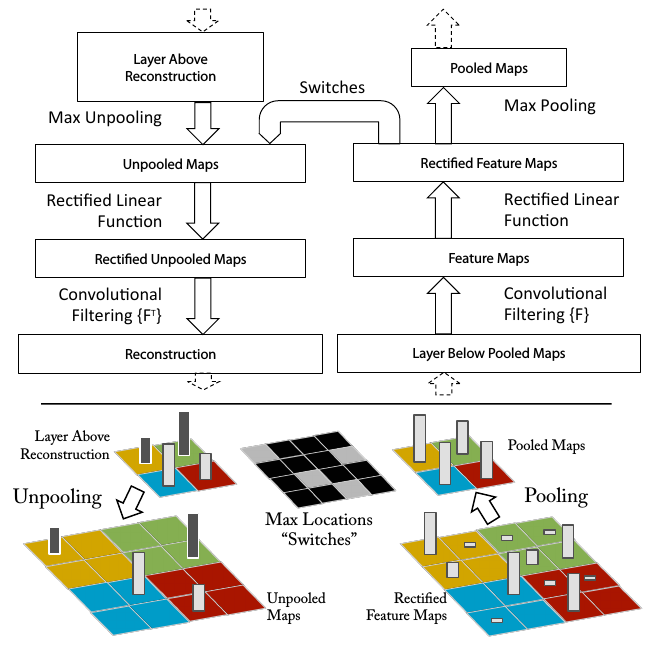
\includegraphics[width=8cm]{Images/deconv}}
		\caption{Deconvolution Process}
		\label{deconv}
	\end{figure}
	
	
	\section{Evaluations}
	\subsection{Dataset}
	The original AlexNet and ZFNet were trained on ImageNet dataset [4] which comprises of 1.2 million images from 1000 different categories. As mentioned by the authors themselves training AlexNet took about 6 days, whereas ZFNet took around 12 days to train. Because of lack of availability of computational power and time I had to go for a much smaller dataset for training the convnets. I have trained both the models using \textbf{Caltech-101} [3] dataset which contains image from 101 different categories with 40 to 800 images of each type. The size of each image is roughly around $300 \times 200$ pixels. 
	
	\subsection{Training ConvNets}
	Initially, for training the convnets I had to struggle through a lot of unsuccessful attempts because of irregular choice of parameters. One such unsuccessful attempt is shown in Figure \ref{c_train}, as we can see from the figure that the test loss is drastically increasing with epochs which indicates that the training is going in the wrong direction. This was mainly because of the high learning used for training. 
	
	\begin{figure}[h]
		\centering
		\fbox{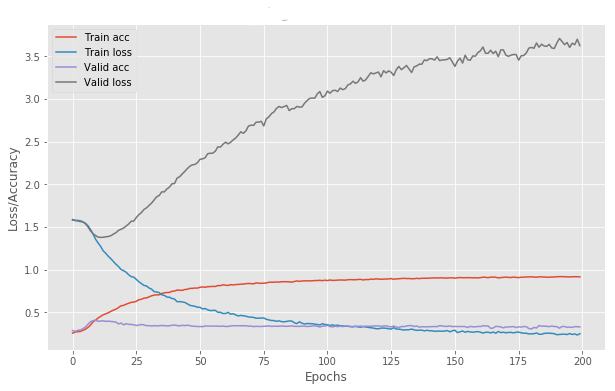
\includegraphics[width=12cm]{Images/c_train2}}
		\caption{Unsuccessful training}
		\label{c_train}
	\end{figure}
	
	Finally, The both the convets (AlexNet, ZFNet) were successfully trained and it took around 6 hours for the training to reach convergence for both the networks. The following are the accuracy and loss plot for training and test data with epochs. Both the networks attained \textbf{100 \%} accuracy on training data and on test data AlexNet achieved an accuracy of \textbf{74.06 \%}, whereas, ZFNet attained an accuracy of \textbf{74.69 \%}.
	
	
	\begin{figure}[h]
		\centering
		\fbox{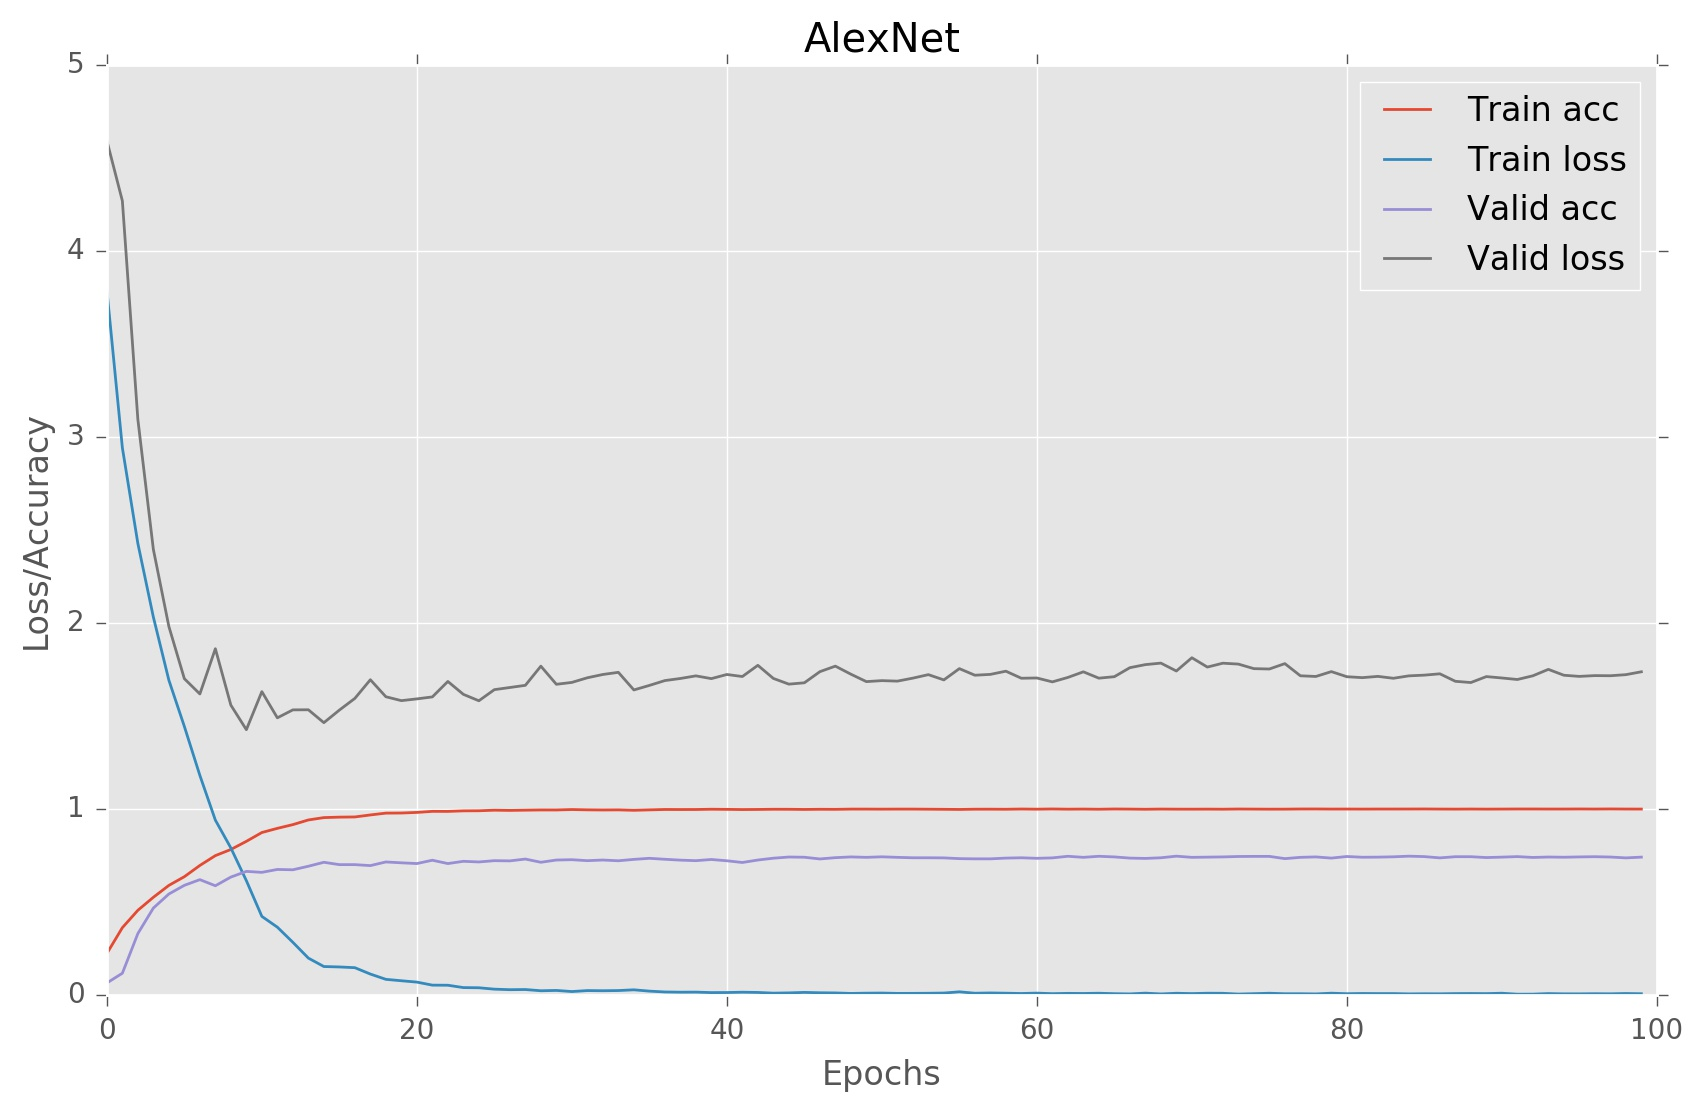
\includegraphics[width=12cm]{Images/alex_train}}
		\caption{\textbf{Training AlexNet}}
	\end{figure}

	\begin{figure}[h]
		\centering
		\fbox{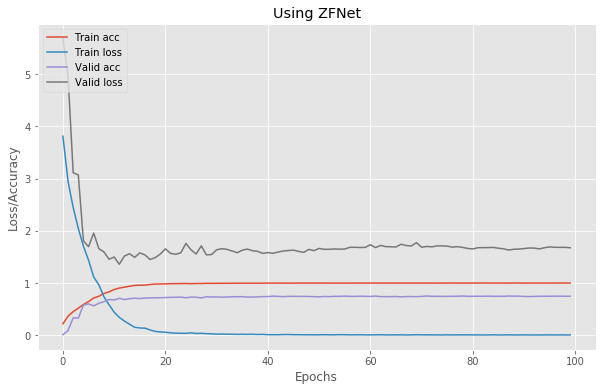
\includegraphics[width=12cm]{Images/zfnet_train}}
		\caption{\textbf{Training ZFNet}}
	\end{figure}


	\newpage	
	\subsection{Visualizing ConvNets}
	The visualization of the activation of the convolution layers of AlexNet and ZFNet for the input image (Figure \ref{viz_input}) are shown below. For each convolution layer of the architectures its first 100 outputs and the deconvolution results have been displayed. Based on these results only Zeiler and Fergus proposed a correction to AlexNet architecture which lead to ZFNet. We can see from the deconvolution results of AlexNet's layers that there are block artifacts in them, which are making it to mispredict on several test instances. This problem can be addressed by reducing the size of the filters and stride used in convolution layers which will give us the results of ZFNet model. This change drastically improves the performance of AlexNet.
	
	
	\begin{figure}[!htb]
		\centering
		\fbox{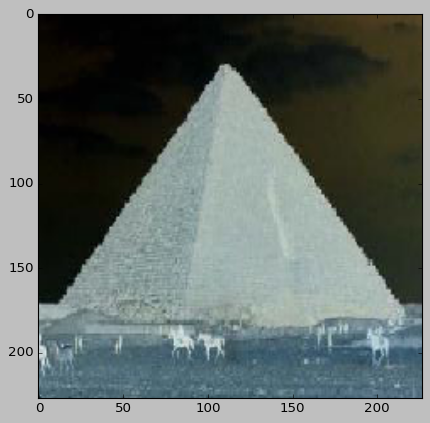
\includegraphics[width=4cm]{Images/viz_alex/alex_input}}
		\caption{Input Image for Visualization}
		\label{viz_input}
	\end{figure}

	\begin{figure}[!htb]
		\centering
		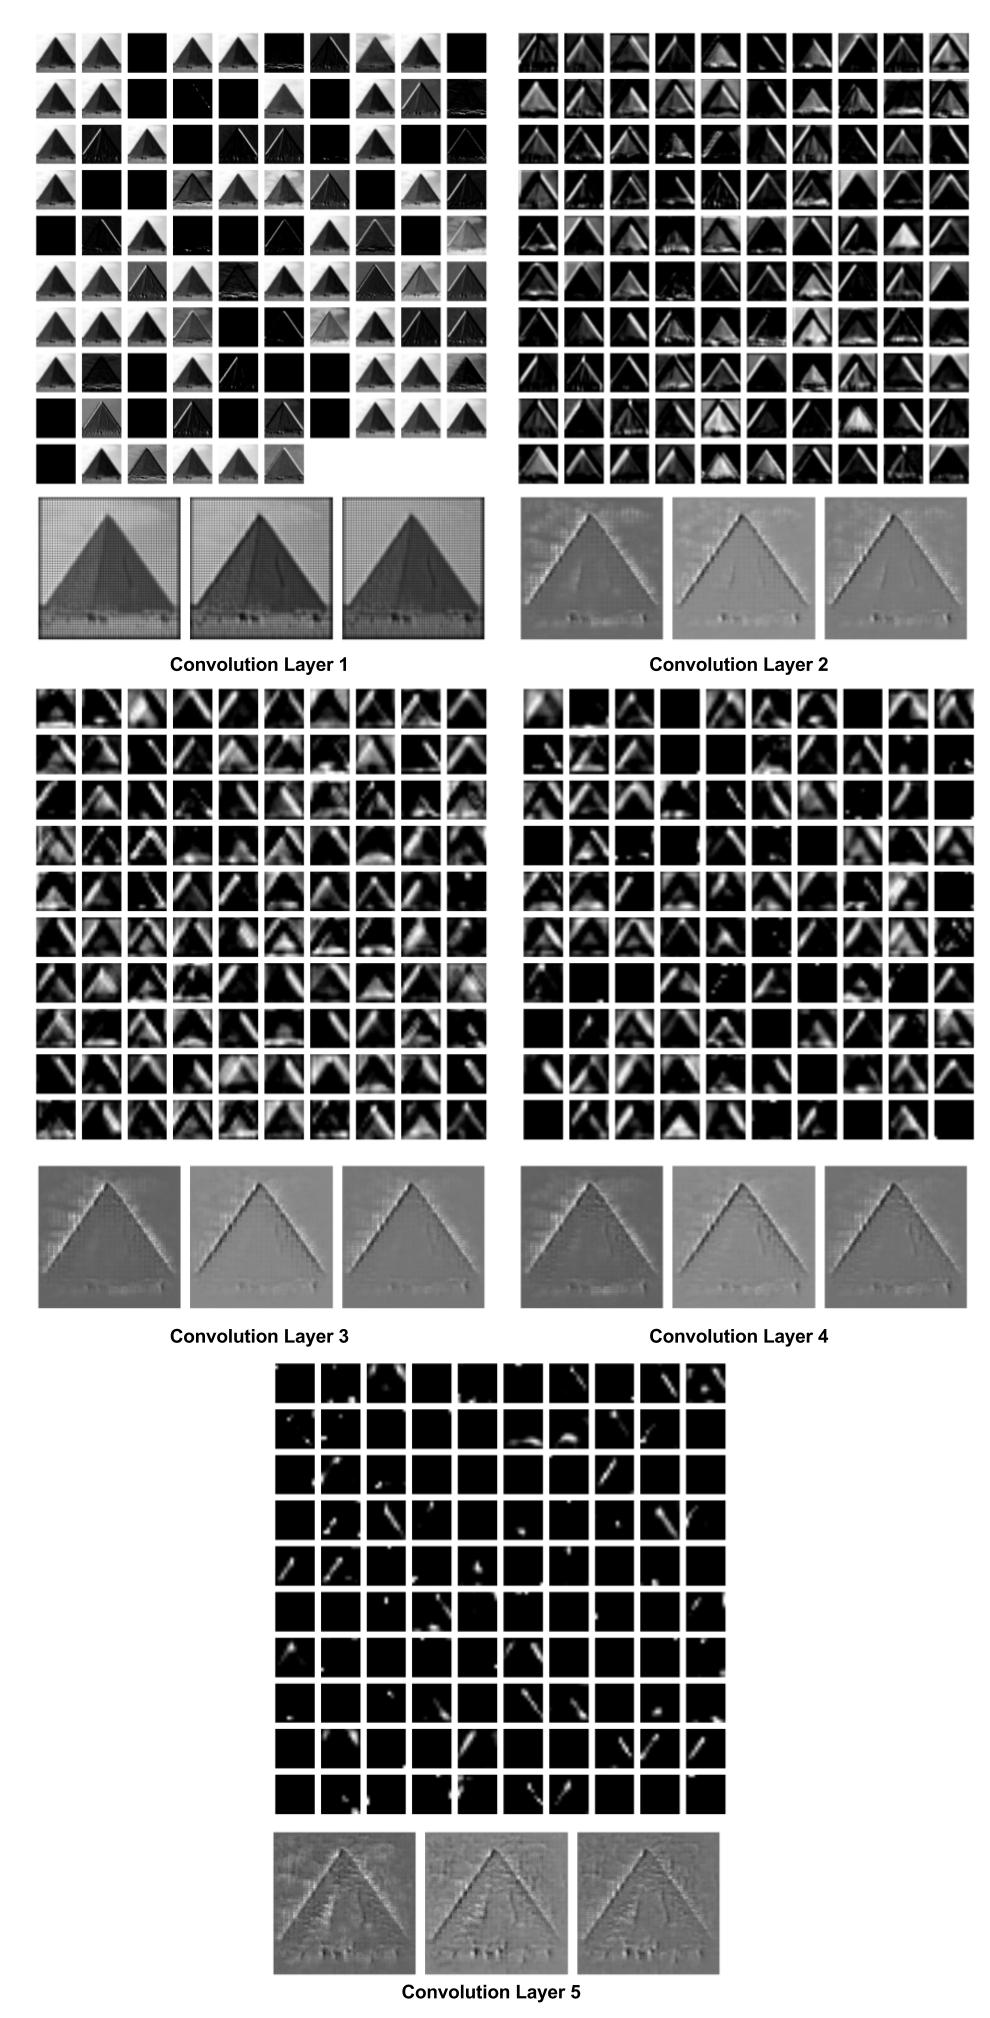
\includegraphics[width=10cm]{Images/Alex_Viz}
		\caption{\textbf{Visualizing AlexNet architecture}; For each convolution layer, the images shown in 10x10 array is the output of the layer and the three images below it shows the three channels of the projected activation of the layer obtained using Deconvolution}
	\end{figure}

	\newpage
	\begin{figure}[!htb]
		\centering
		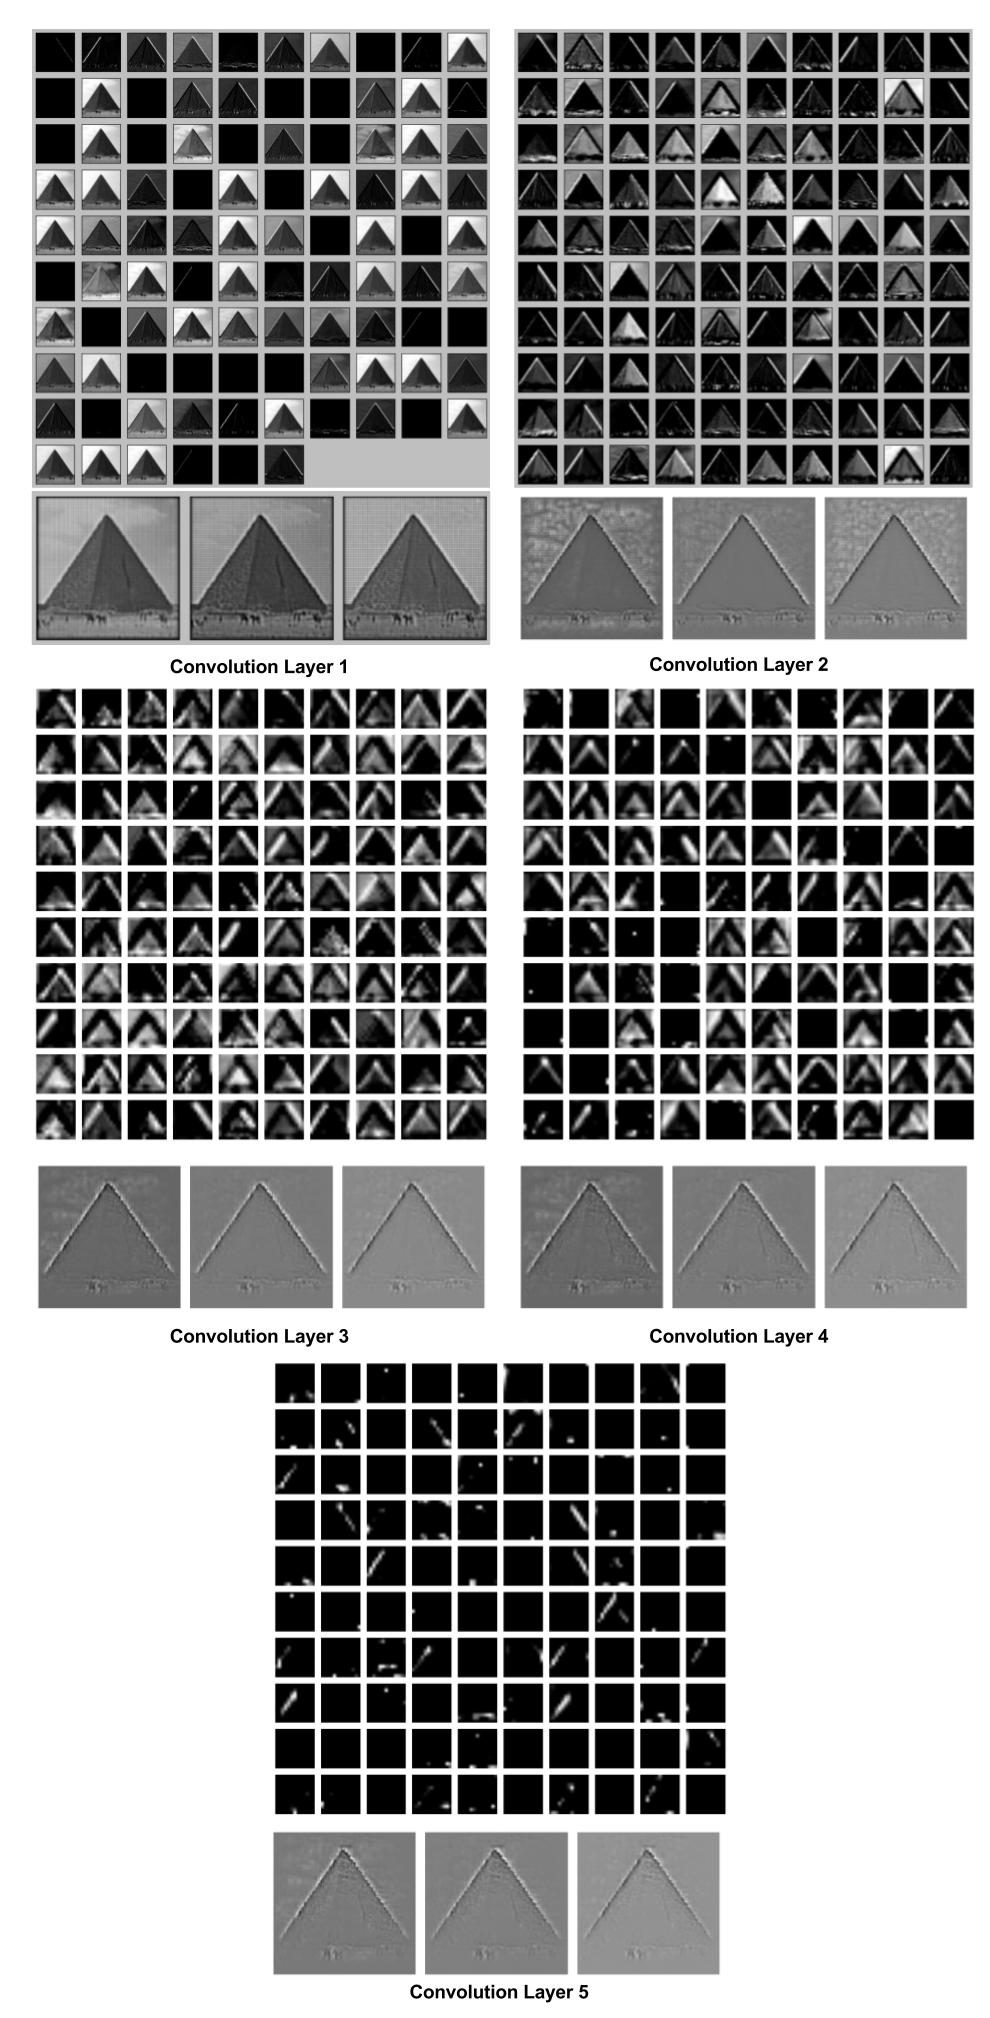
\includegraphics[width=10cm]{Images/ZFNet_Viz}
		\caption{\textbf{Visualizing ZFNet architecture}; For each convolution layer, the images shown in 10x10 array is the output of the layer and the three images below it shows the three channels of the projected activation of the layer obtained using Deconvolution}
	\end{figure}

	\newpage
	\section{DeNet - A new method for visualization}
	The method proposed by Zeiler and Fergus only allows us to visualize the activation of convolution layers, but instead of constraining ourselves to that we can also look for visualizing the summary of the activation captured by the entire ConvNet. I have come up with a method which allows us to highlight the features in an image which play the most important role in making it associated with a particular category. The technique could be called as \textbf{Decode ConvNet} or \textbf{DeNet} in short. DeNet helps us to understand how ConvNets are extracting pattern from the images. The method begins with a vector containing the class information of an image in one-hot encoding format. Then, starting from the final output layer of the ConvNet, the vector is shoved towards the input layer through all the layers of the network. At Dense layer, the tensor is multiplied by the transpose of the weight matrix used during the forward pass after subtracting the bias. At Convolution and pooling layers, the deconvolution and unpooling operations are used as proposed in [5]. This finally leads the class-vector to the pixel domain where the results can be visualized easily. 
	
	Using the above proposed technique, I tried to compare AlexNet and ZFNet architectures and obtained the following results. We can see in the Figure \ref{denet}, the problems with AlexNet architecture. The blocks artifacts in the activation are clearly visible which negatively affects its classification accuracy, such artifacts are not visible in ZFNet model. Moreover, ZFNet is able to capture more details of the image as compared to AlexNet, the face category results clearly shows this fact. The face in the case of ZFNet is much more clear and sharp as compared to what is being extracted by AlexNet. Same is the case with other categories as well. 
	
	\begin{figure}[!htb]
		\centering
		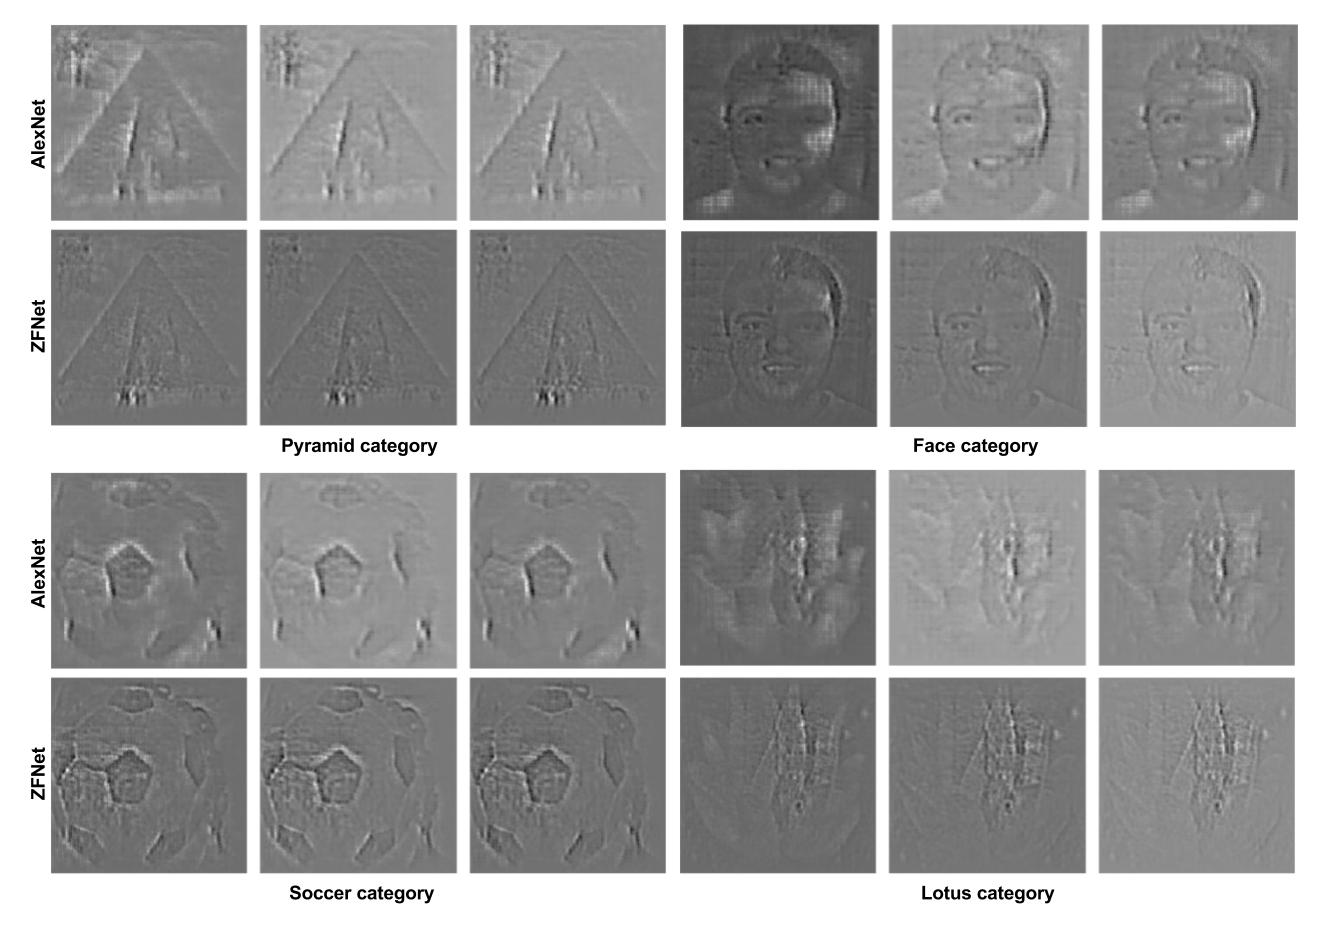
\includegraphics[width=14cm]{Images/denet/denet}
		\caption{\textbf{Results with DeNet Visualization}}
		\label{denet}
	\end{figure}

	\section{Comparing DeNet with Deconvolution}
	Figure \ref{denet_comp} shows the comparison of DeNet with Deconvolution technique proposed by Zeiler and Fergus [2]. From the results it is clearly evident that the proposed method is more effective in capturing the features extracted by the ConvNets than Deconvolution. Thus, it can be more helpful in visualizing ConvNets. The better performance of DeNet is because of the fact that it extracts information even from the dense layers of the network, which is completely ignored by Deconvolution method. 
	
	\begin{figure}[!htb]
		\centering
		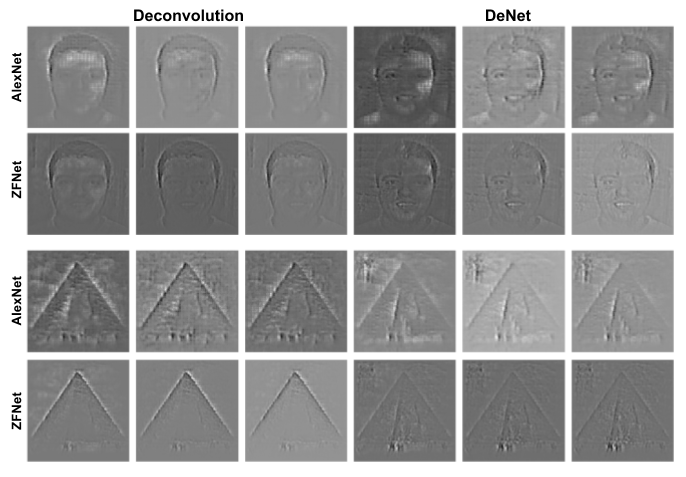
\includegraphics[width=14cm]{Images/DeNetComp.png}
		\caption{\textbf{Comparing DeNet with Deconvolution}}
		\label{denet_comp}
	\end{figure}
	
	\section{Conclusion}
	The project looks into the working of two Convolution Neural Netwoks, AlexNet and ZFNet and explores the evolution of the former from the later. It helps to understand that how the hyperparameters of CNNs can be set and corrected scientifically by visualizing the activation of ConvNet layers. It demonstrate the visualization every layer of AlexNet and ZFNet architecture trained using Caltech-101 dataset through deconvolution and also proposes a novel way of visualizing features extracted by a ConvNet for a given image using a technique called DeNet.
	
	\subsubsection*{References}
	
	\small{
		[1] Krizhevsky, Alex, Ilya Sutskever, and Geoffrey E. Hinton. "Imagenet classification with deep convolutional neural networks." Advances in neural information processing systems. 2012.
		
		[2] Zeiler, Matthew D., and Rob Fergus. "Visualizing and understanding convolutional networks." European conference on computer vision. Springer International Publishing, 2014.
		
		[3] Olga Russakovsky*, Jia Deng*, Hao Su, Jonathan Krause, Sanjeev Satheesh, Sean Ma, Zhiheng Huang, Andrej Karpathy, Aditya Khosla, Michael Bernstein, Alexander C. Berg and Li Fei-Fei. (* = equal contribution) ImageNet Large Scale Visual Recognition 
		
		[4] L. Fei-Fei, R. Fergus and P. Perona. Learning generative visual models
		from few training examples: an incremental Bayesian approach tested on
		101 object categories. IEEE. CVPR 2004, Workshop on Generative-Model
		Based Vision. 2004
		
		[5] Zeiler, Matthew D., et al. "Deconvolutional networks." Computer Vision and Pattern Recognition (CVPR), 2010 IEEE Conference on. IEEE, 2010.
	}
	
\end{document}